\section{Evaluation}
\label{s:evaluation}
% table of workload characteristics
\begin{table*}
\centering
\label{table:workloads}
\caption{Workload attributes. The \textit{Runtime} column refers to the featurization update runtime for a single key. The \textit{Min Loss} and \textit{Max Loss} columns show the overall loss given infinite budget and zero budget for featurization, respectively. The minimum loss for the Azure dataset is shown in \cref{f:stl-time}. }
\begin{tabular}{|l|l|l|l|l|l|l|l}
\cline{1-7}
\textbf{Workload} & \textbf{Dataset} & \textbf{Keys} & \textbf{Runtime} & \textbf{Edits}  & \textbf{Min Loss} & \textbf{Max Loss} &\\ \cline{1-7}
Recommendation & MovieLens 1M & 6041 & 0.9s & 85,297 & 1.12 & 6.29 & \\ \cline{1-7}
%IR & Wikipedia Edits & 200 & 1.1s & 16,342 & 75.3\% & 94.3\% &  \\ \cline{1-7}
 & Yahoo Anomaly A1  & 68 & 0.25s & 43,684 & 90.79 & 880.3 & \\ \cline{2-7 }
\multirow{-2}{*}{\begin{tabular}[c]{@{}l@{}}Time-Series \\ Decomposition \end{tabular}}  & Azure VM Dataset  & 275,077 & 0.4 & 5,683,390 & - & - & \\ \cline{1-7}
\end{tabular}
%\vspace{-2em}
\end{table*}

In this section, we address two primary questions: (1) how does Regret-Proportional scheduling impact downstream prediction accuracy (2) how does \system{} with Regret-Proportional scheduling scale to processing high-cardinality, high-rate data streams? To answer these questions, we structure our evaluation as following:
\begin{enumerate}
    \item We construct representative workloads for two common feature store use-cases, recommendation and anomaly detection, using real-world datasets. For both workloads, we evaluate feature quality by evaluating model predictions that rely on feature which are updated over time. 
    \item We run an end-to-end evaluation with \system{} on a large-scale anomaly detection workload to evaluate prediction accuracy improvements, system overhead, and scaleability. 
    \item We run ablations comparing Regret-Proportional scheduling with both baseline and application-specific policies. 
\end{enumerate}



\subsection{Workloads} 
\label{ss:workloads}

%\noindent\textbf{Workload Generation.}
\label{ss:evaluation:workloads}
To evaluate feature maintenance policies, we construct workloads using real-world data where model predictions rely on pre-computed features that need to be updated as new events are streamed in. For each workload, we use real-world data to generate an \textit{update stream} (incoming raw data),  \textit{query stream} (queries from downstream models), and \textit{feedback stream} (error feedback). 

For each workload, we setup to following components to mimic realistic prediction serving applications: A  \textbf{feature function} (the operator that transforms data streams into features cached in the feature table), \textbf{feature table} (the key/value store contained feature keys and values), and \textbf{downstream model} (the downstream prediction serving application which queries feature table values that are used to make predictions). 

We describe the dataset, featurization, and downstream models for recommendation and anomaly detection workloads. A summary of workload attributes is show in \cref{table:workloads}, which also shows the best and worst-case prediction loss depending on feature quality. 


\subsubsection{Anomaly Detection}


Time series decomposition is a common pre-processing step to many downstream tasks, such as anomaly detection or forecasting. We construct an time-series anomaly detection workload based off a real-world application at Splunk \cite{wang2021online,mishra2021onlinestl}. The anomaly detection task compares predicted points from time-series features, calculated from windows of past data, with the observed points to detect anomalies. Accurate anomaly detection depends on estimating the residual of the point accurately, which relies on the accuracy of the cached time-series features. The \textit{query stream} periodically queries all keys to detect anomalies in regular time-intervals, so the distribution of queries over keys is uniform. Features are maintained over an \textit{update stream} of new time-series points. Each new time-series point is compared to previously predicted points to provide a \textit{feedback stream}.

\myparagraph{Dataset}
We use both the Yahoo Webscope S5 Dataset's A1 class \cite{laptev2015yahoo} and Azure VM dataset \cite{cortez2017resource}.\sarah{I could have both teh graphs for yahoo and azure, but they look the same...} We use the Python statsmodels library \cite{seabold2010statsmodels} to compute features from windows of data for each time-series. For the Yahoo dataset, the rate of updates and start time for each time-series is uniform across keys, so the distribution of queries and feedback across keys is also uniform. However, the variation in the time-series can vary dramatically across keys, opening opportunity for optimizing resource allocation across keys. For example, some time-series vary little over time, while others change rapidly and have complex and variable seasonality components. \sarah{add example time-series?}

% new for the revision, more description about the Azure dataset - simon



%\myparagraph{Scheduling Policies} We implement a baseline policy as a round-robin policy (\textit{roundRobin}) which iterates over keys to choose which key to update next. We also implement our scheduler described in \cref{ss:online-scheduling-error-feedback}, which we refer to as the \textit{regret optimized} scheduling policy. Altough the staleness of the queried keys is minimized by the round robin policy, as shown in \cref{fig:stl-yahoo-staleness}, minimizing feature staleness does not necessarily minimize prediction loss. We show the average error across keys in \cref{fig:stl-yahoo-error}, where the regret optimize has significantly lower average prediction loss across queries as compared to round-robin. The regret optimized scheduler is able prioritize keys which are more likely to degrade prediction accuracy using error feedback. We show in \cref{f:stl-a1-heat} the most frequently updated keys by the regret optimized scheduler, and the corresponding number of updates for the same keys by the round robin scheduler. 


\subsubsection{Recommendation}

Recommendation is another applications where machine learning models are used to make low-latency recommendations to users, often using user features derived from historical data to personalize predictions. We construct a recommendation workloads where a downstream models predicts what a user's rating for a movie will be user and movie features computed from past rating data, where user features are updated online. Given a stream of user ratings for movies, we simulate a \textit{query stream} over the users to predict what the rating should be. We return the prediction error of the rating as the \textit{feedback stream}, and treat the rating itself as data update from the \textit{event stream}. The incoming event stream of ratings is used to update user embeddings over time using partial ALS to update the corresponding feature vector. 

\myparagraph{Dataset}
We use the MovieLens 1M \cite{movielens1m}, which has timestamped ratings from roughly a million user/movie pairs. We use the first half of the data to train a model using Alternating Least Squares\sarah{cite?}. We treat the resulting movie embeddings as the static \textit{model} and the user-ratings as \textit{features} which are updated over time. We use the second half of the data as query, event, and feedback streams. 

%\myparagraph{Scheduling Policies} In addition to round robin, we implement two additional natural baseline policies: 1. selecting the key with the maximum pending updates (\textit{maxPending}), 2. selecting the key with the fewest observed data points (\textit{minPast}). We also implement our regret optimize policy using the error feedback from the rating predictions. We find that \textit{minPast} and \textit{regret} perform significantly better than other policies, as they prioritize updating users with the least amount of prior information. For more resource constrained settings, we find that \textit{regret} still performs substantially better than  \textit{minPast}. For keys updated the most frequently by round robin, we show the number of updates allocated by other policies in \cref{f:als-heat}. Due to variation the number of users receiving updates over time, the distribution of updates is similar between policies. However this slight variation in updates is enough to dramatically affect accuracy.




%Time series decomposition is a common pre-processing step to many downstream tasks, such as anomaly detection or forecasting. We construct a time series decomposition featurization pipeline based off real-world workloads at Splunk. Time-series data from many different sources decomposed into trend and seasonality components. These trend and seasonality estimates can be used to evaluate the \textit{residual} (or noise) of later points in the time-series, which can be used for anomaly detection tasks. 

%We evaluate the state of the feature store based off the quality of the \textit{residual estimates} of the downstream task. The downstream anomaly detection task calculates a residual for each new point for each time-series by querying the time series ID from the feature table to obtain the time series' features. We use the loss of the residual estimate to evaluate the features, using the residual calculated from fitting the STL model to the entire dataset as the "ground truth" residual estimate. We generate a query pattern which regularly queries all keys in the feature store to generate residual estimates (for anomaly detection) for all keys. 

 

\subsection{End-to-End Evaluation}
% Full Azure Figure 
\begin{figure*}[t]
\begin{center}
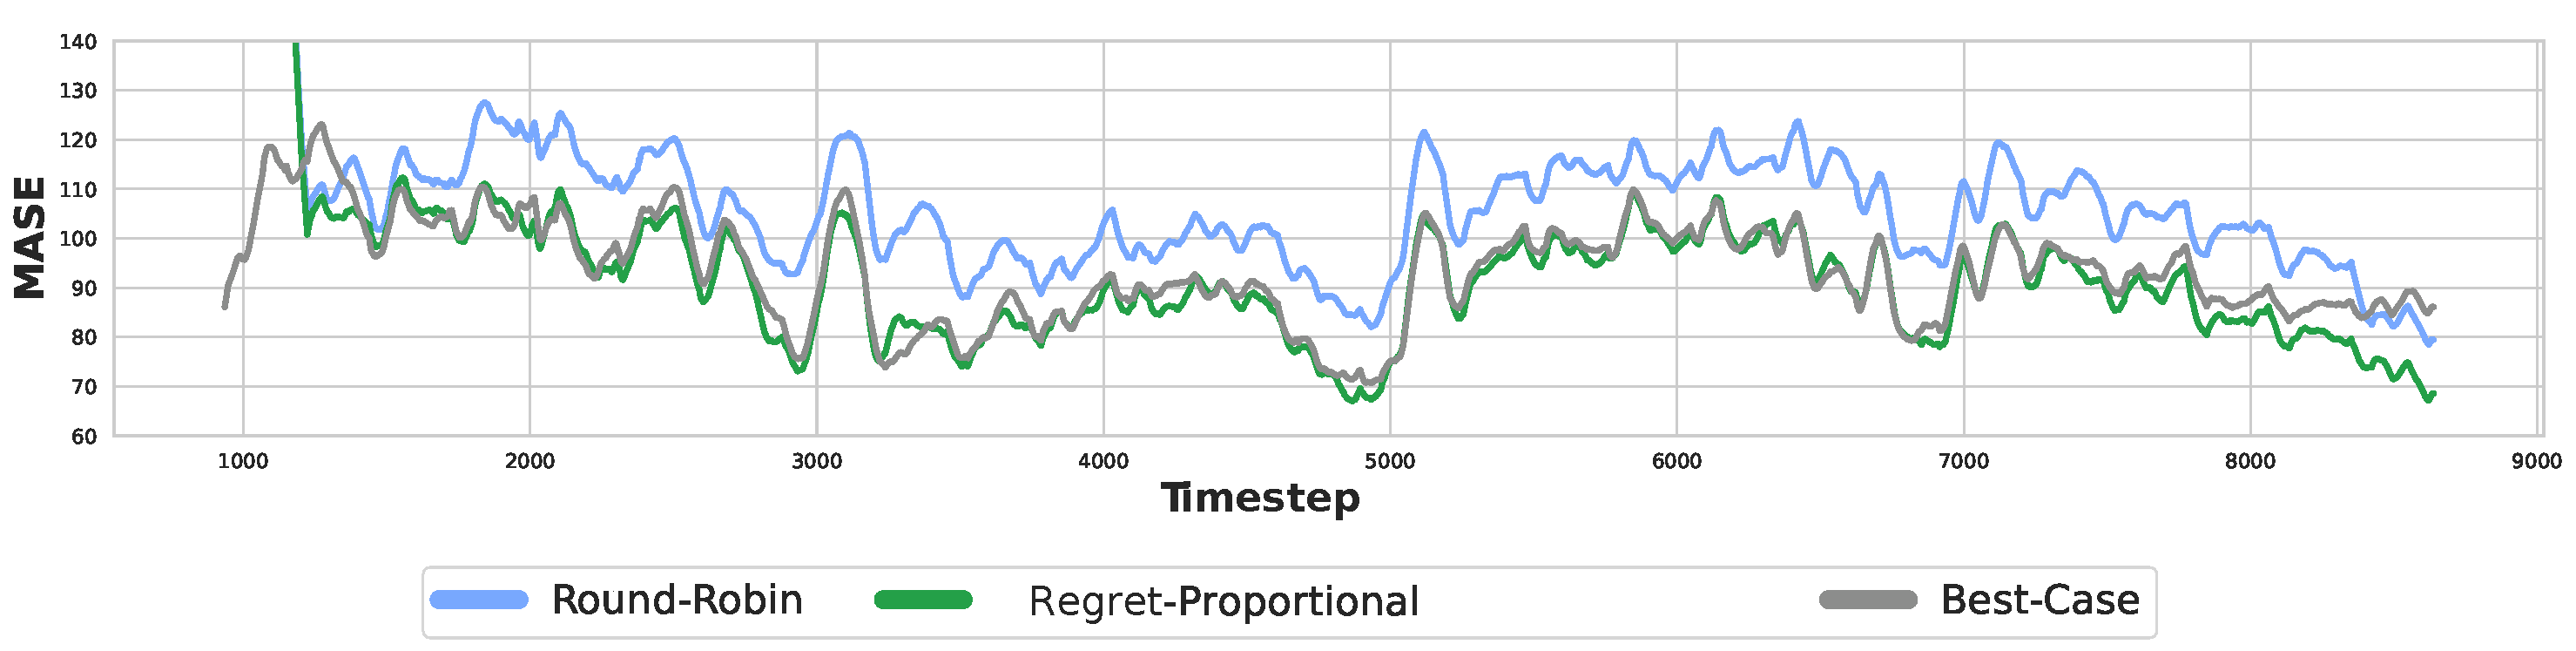
\includegraphics[width=15cm]{ralf/figures/ralf_azure.pdf}
\centering
\end{center}
\caption{Smoothed Average MASE per Timestep over 275,077 keys.
%We calculate MASE across all 275,077 keys at each timestep for the Regret-Proportional, Round-Robin, and Best-Case features. The Regret-Proportional policy closely matches error as if we have infinite resources. Compared to the Round Robin policy, Regret-Proportional policy averages to 13.3\% and peak at 32.7\% error improvement.
}
\label{f:stl-time}
\end{figure*}

We evaluate \system{} on 800 cores for end-to-end with the Anomaly Detection workload using the Azure VM dataset \cite{cortez2017resource}. We run \system{} with both our Regret-Proportional policy and baseline policy of Round-Robin scheduling to evaluate prediction accuracy, scheduling overhead, and scaleability.  

\subsubsection{Experimental Setup}
The Azure VM dataset includes of the CPU readings taken every 5 minutes on a pool of 2 million VMs over the span of one month. We send a subsample of 275,077 time-series from Azure Dataset on a cluster of 11 m5d.24xlarge machines (800 cores) on AWS. We simulate higher data send rates by sending at 1000x speed (i.e. ingesting data once every 0.3 seconds, rather than every 5 minutes as specific in the dataset). We use \system{} to compute an STL decomposition of the time series for each key, using a recent observation window. We set the STL decomposition seasonality to be 24 hours, and set the observation window size of data to be 3X the seasonality length (so 72 hours of recent data points) to have a sufficiently large window to compute the decomposition. We store the resulting STL decomposition as a feature in the feature store for each key (i.e. a time-series ID), which is updated over time by \system{} as new data arrives. Because of the high data rate, some features will be out of date with the current observation window. \system{} uses either the Regret-proportional or Round-Robin scheduling policy to choose which features to prioritize updating.

\subsubsection{Policy Error}
To evaluate feature quality, we compare the MASE (Mean Absolute Squared Error) of time-series predictions using the STL decomposition features using the Regret-Proportional and Round-Robin scheduling policies in \cref{f:stl-time}. We can calculate the MASE by comparing the predicted points with the actual points observed. We show a plot of average MASE across keys over time for features computed with the Regret-Proportional and Round-Robin scheduling policies in \cref{f:stl-time}.  Although overall MASE varies over time, the Regret-Proportional policy consistently produces lower MASE than the Round-Round policy features, with error improvement ranging from 2-32.7\% and averaging to 13\%.

We additionally calculate the \textit{optimal} version of the features (described in \cref{ss:regret}) for each query by calculating what the feature value would be with all data up to exactly the query time. The optimal features correspond to the best case MASE (shown in grey in \cref{f:stl-time}) enabled by unlimited compute resources (i.e. processing every possible update). We see that the MASE for optimal features and the Regret-Proportional policies are similar in \cref{f:stl-time}. The Regret-Proportional policy over the course of the experiment runs 61\% fewer updates (i.e. $1.6\times$ less) than would be needed to achieve the optimal features, however averages only 1\% additional error as compared to optimal features. 

%Infinite resource is simulated because it takes ~2x the resource as compared to both policy. On full scale of the the Azure Dataset, Regret Optimized policy only needs to evalaute 61\% of the windows to match the error (with 1\% penalty) of using evaluating all the windows.

\subsubsection{Scaling Evaluation}
We evaluate how \system{}'s throughput scales in  \cref{f:stl-throughput} by measuring the throughput per number of cores for Round-Robin versus Regret-Proportional scheduling. For both the Round-Robin and Regret-Proportional policies, the throughput scales linearly with the number of cores. Because the workload is embarrassingly parallel, we can shard keys across replicas, where each replica corresponds to one core and has its own scheduling and transformation operator. As a result, the number of updates scales linearly with with the number of cores. We use randomized hashing to place keys on replicas and utilize 800 cores of workers.

\begin{figure}[t]
\begin{center}
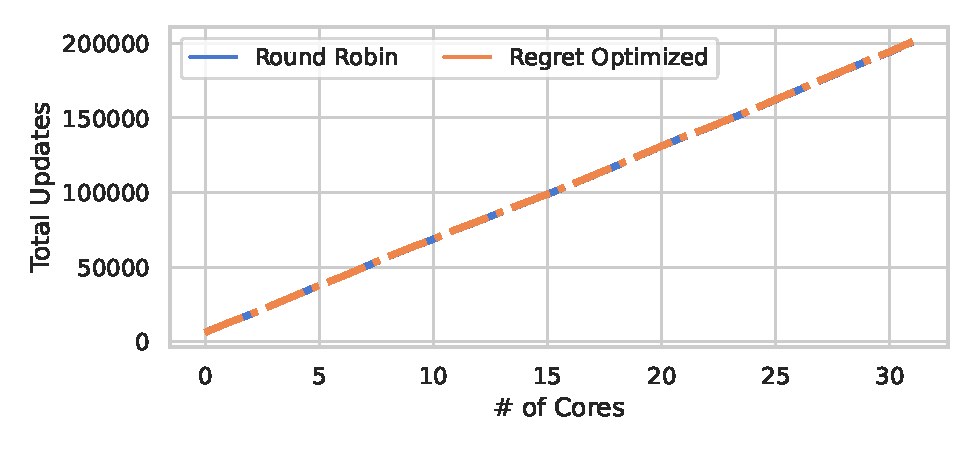
\includegraphics[width=6cm]{ralf/figures/scaling-april-15-10k-keys.pdf}
\centering
\end{center}
\caption{System throughput versus number of cores.}
%\textcolor{red}{TODO: potentially add graph of time in scheduling, workload breakdown, number of updates difference. Add memory size? Throughput per core?}
\label{f:stl-throughput}
\end{figure}

\subsubsection{Scheduling Overhead}
\label{s:overhead}
%We observe about a $1\%$ overhead with Regret-Proportional scheduling compared to Round-Robin, however this overhead is constant with respect to the number of cores, as shown in \cref{f:stl-throughput}. 

We evaluate the scheduling overhead of Regret-Proportional versus standard Round-Robin scheduling in terms of both compute and memory. The Regret-Proportional policy requires  a constant CPU cost of 300 $\mu s$ per arrived window queued for update in order to evaluate the regret score. Furthermore, maintaining a sorted queue (ordered by per-key regret) costs 50 $\mu s$ per addition/removal. Additionally, because the regret calculation requires previous feature to be cached in memory, the Regret-Proportional policy also costs about 32 KBs per key, resulting in about 11MB of memory overhead per core. We note that the per-core compute and memory overhead is constant regardless of the number of cores used, due to scheduling occurring per-replica rather than globally. This allows us to mitigate coordination overhead and is sufficient for making scheduling decisions that load balance across threads and optimize feature quality. 

%The overhead is fairly small and does not increase with scaling as \system{}'s scheduler is run each individual worker instead of using a global scheduler. 

%With large enough keys to prioritize within the worker, the localized scheduling decisions closely resemble those of a global scheduler. For example, in the previous scaling experiment on 800 cores, each worker gets to schedule the computation over ~350 keys. 

We plot the total throughput as a function of total cores in \cref{f:stl-throughput}. The Regret-Proportional policy performed 0.6\% less updates as compared to Round-Robin policy. However, despite fewer number of updates performed, the cached features from Regret-Proportional scheduling results in significantly better model performance. This is because the Regret-Proportional policy can achieve similar feature quality with dramatically fewer updates, as shown by achieving near-optimal feature quality with 61\% fewer updates.




\begin{figure*}[t]
     \centering
    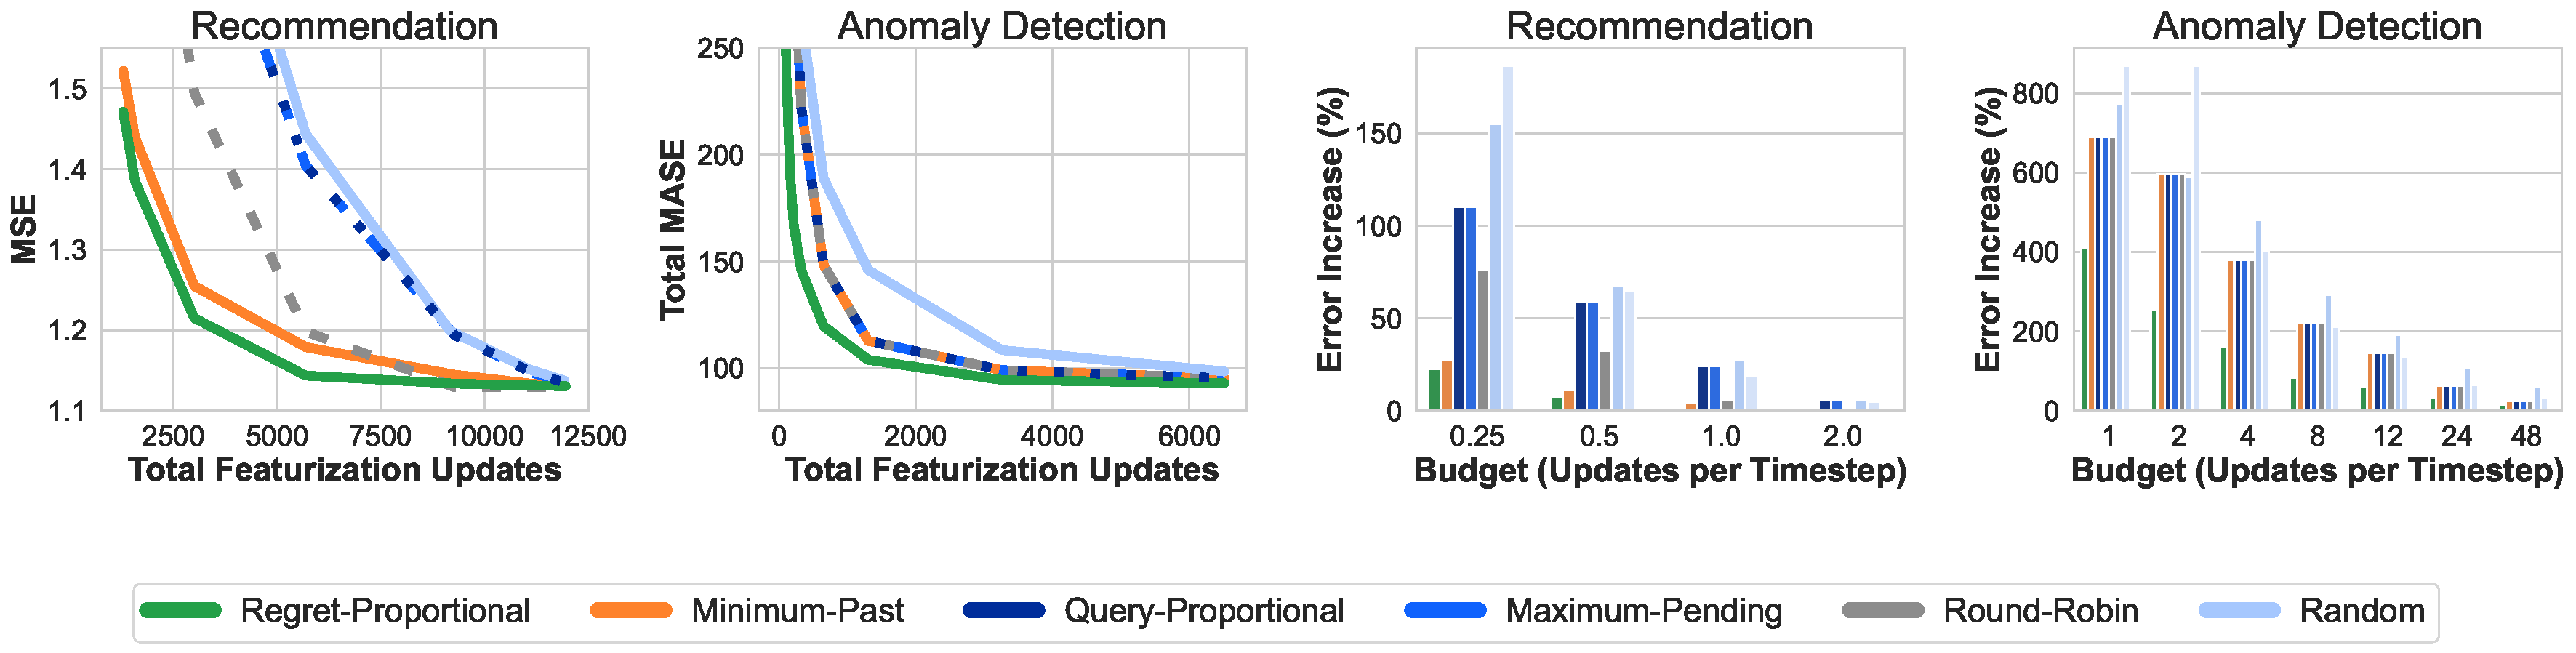
\includegraphics[width=17cm]{ralf/figures/line_all_no_ir.pdf}
    \caption{Left: Prediction error versus total featurization updates (over the entire experiment). Right: Error increase (compared to optimal features with unlimited budget) for varied update budgets.}
    \label{fig:results-all-line} 
\end{figure*}

\subsection{Policy Ablations}
We compare the Regret-Proportional scheduling policy to other baseline and application-specific policies that do not consider downstream prediction accuracy. We run simulated experiments with both the Recommendation workload and the Anomaly Detection workload (using a smaller time-series dataset, the Yahoo A1 dataset) to show the generality of our policy improvements.  
\label{s:policy-evaluation}


\subsubsection{Policies}
We implement the \textbf{Regret-Proportional} policy described in \cref{ss:online-scheduling-error-feedback}. Similarly, we implement a \textbf{Query-Proportional} policy which updates features proportionally to the rate they are queried (i.e. the number of times the feature has been queried since last updated), to understand the impact of regret versus query awareness.  We evaluate these policies along with baseline query-oblivious policies commonly found in stream processing systems. 


We implement baseline query-oblivious policies for choosing which keys to update: 
\begin{itemize}
    \item \textbf{Round-Robin}: Iterate over each key and skip keys with no pending updates (equivalent to updating the most stale and least-recently-updated key). 
    \item \textbf{Random}: Randomly select a key with pending updates. 
\end{itemize}
We additionally implement two more sophisticated query-oblivious policies designed to improve accuracy in the Recommendation workload:  
\begin{itemize}
    \item \textbf{Minimum-Past}: Update keys that have the least data incorporated into the feature (i.e. the number of ratings seen for the user). 
    \item \textbf{Max-Pending}: Update keys with the most pending new data (i.e. the user with the most new ratings).
\end{itemize}



\subsubsection{Prediction Error }

To evaluate the quality of features derived with different policies under different cost constraints, we simulate the policies for each workload.  
%
At each timestep in the simulation, there is a set of feature update events and feature queries for a set of prediction at that timestep. 
%
We set an update budget, which limits the number features we can update per timestep. 
%
The subset of features to update is chosen by the scheduling policy. 
%
At each timestep, the simulator processes some subset of feature updates chosen by the scheduler and generates predictions using the current set of features, which we use to evaluate error in \cref{fig:results-all-line}. 

%The features are used to evaluate the overall prediction error incurred over time, which we use to compare the results of different policies.
%
\subsubsection{Regret-Proportional Policy}
The Regret-Proportional policy is able to achieve better error across different workloads and numbers of udpates, as shown in \cref{fig:results-all-line}. Query-Proportional updates improves error over baseline policies for the Anomaly Detection workload, as shown in Figure \cref{fig:results-all-line}. However for the Recommendation workload, where it is crucial to update features with little prior data (e.g. new users), the updating proportionally for the queries fails to account for the non-uniform benefit of updates across features. As a result, the Minimum-Past policy, which updates the feature with the fewest prior updates, significantly outperforms the Query-Proportional policy for Recommendation. Weighing the queries by the regret they incur (as in the Regret-Proportional policy) improves the results beyond Query-Proportional updates alone by accounting for \textit{both} the query pattern and the significance of updates. 

%\subsubsection{Minimum-Past vs. Regret Proportional}
New users who have no associated ratings (and hence very poor quality default features) are prioritized by Minimum-Past and Regret-Proportional policies, which significantly improves performance over other policies. However, Minimum-Past cannot distinguish the important of updates between users with similar prior update histories, resulting in worse performance than Regret-Proportional overall. We measure the MSE improvement from the Regret-Proportional policy over Minimum-Past for users with past ratings (Trained) versus new users (Untrained) in \cref{f:user_variance}. Although both policies are similar for new users, the Regret-Proportional policy has substantial improvements over Minimum-Past for existing users keys. The Regret-Proportional policy is able to account for the importance of prioritizing updating new users' features, while also intelligently prioritizing updates across users for which features have already been computed. 


\begin{figure}[t]
\begin{center}
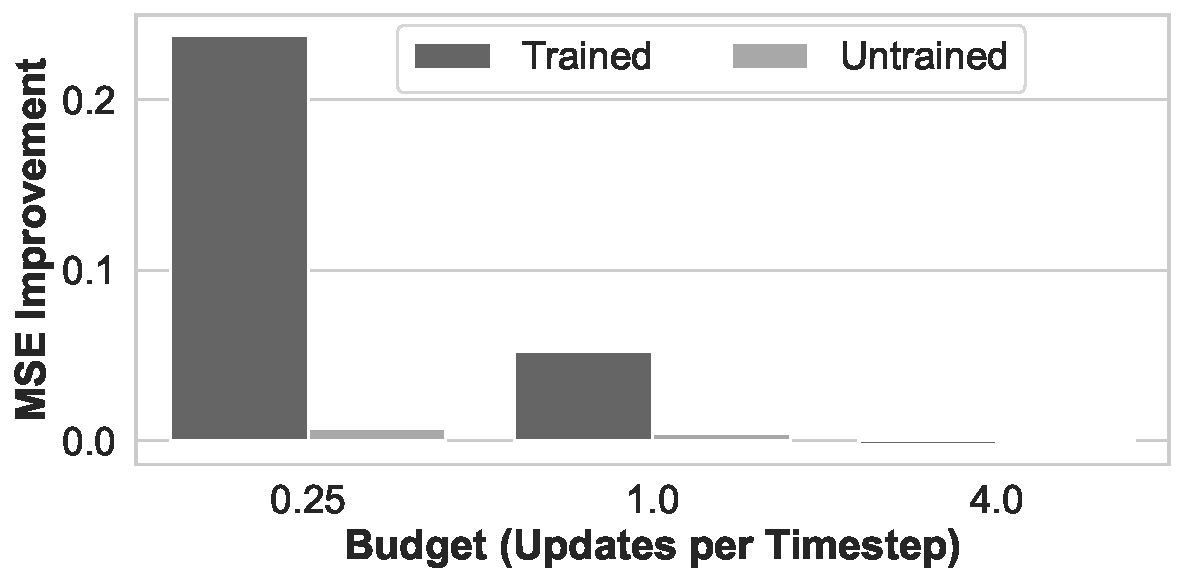
\includegraphics[width=6.5cm]{ralf/figures/user.pdf}
\centering
\end{center}
\caption{Regret-Proportional Improvement over Minimum-Past for users in the training set (Trained) versus new users (Untrained) in the Recommendation workload. }
\label{f:user_variance}
\end{figure}


\subsubsection{Distribution of Updates}
Different policies allocate update budgets in different ways across keys. The variation is most clearly observed for the Anomaly Detection workload, where keys have raw data updates and queries arriving at uniform rates, but are updated with very different distributions depending on the policy, as show in \cref{fig:stl-yahoo-staleness}. The Regret-Proportional policy is able allocate more updates to features incurring regret the most rapidly, resulting in large update variations.


\begin{figure}[t]
\begin{center}
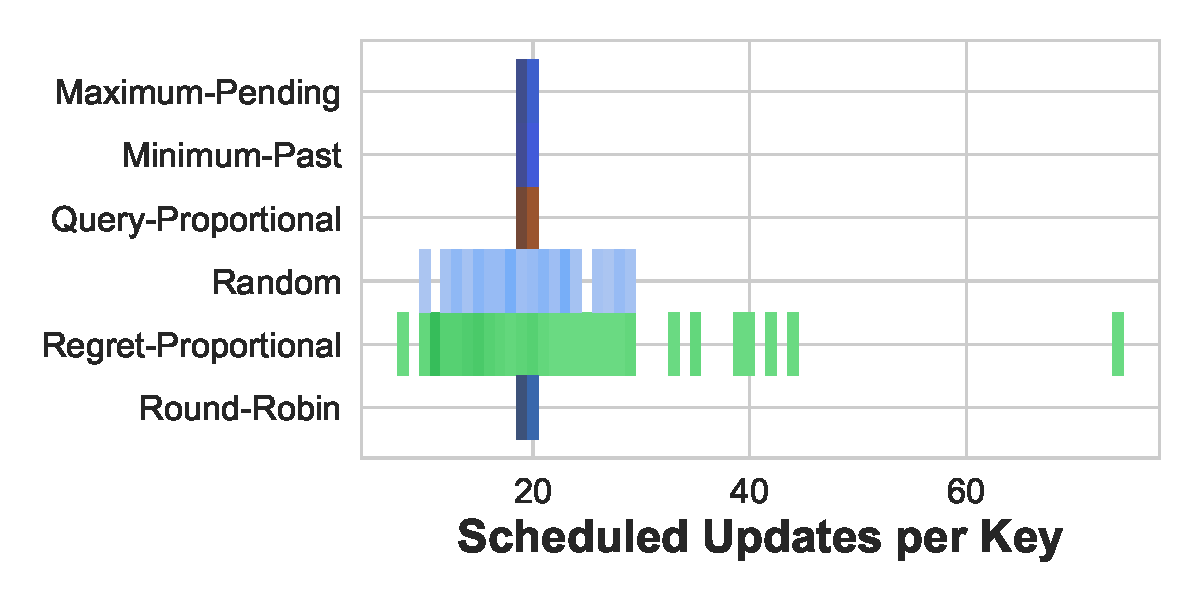
\includegraphics[width=7cm]{ralf/figures/azure_updates_hist_tmp.pdf}
\centering
\end{center}
\caption{\textbf{Distribution of featurization updates (Anomaly Detection):} The Regret-Proportional policy has the most variability in number of updates per key.}
\label{f:update_variance}
\end{figure}

\subsubsection{Optimizing Feature Staleness versus Feature Quality}
Although the staleness of the features is correlated to the prediction accuracy as shown in \cref{f:staleness}, we find that the best performing policies in terms of prediction error are not the best performing in terms of staleness data. As shown in \cref{fig:stl-yahoo-staleness}, the Regret-Proportional has higher average staleness than other policies, including Round-Robin. This is because other policies such as Round-Robin will always prioritize updating the most stale feature, rather than the most important feature to update to optimize downstream prediction error. 
As a result, the Regret-Proportional policy results in better prediction error despite increased staleness, as shown in \cref{fig:results-all-line}. Although staleness is strongly correlated to feature quality, optimizing for staleness does not always have the same results as directly optimizing for feature quality. 

\begin{figure}
    \centering
    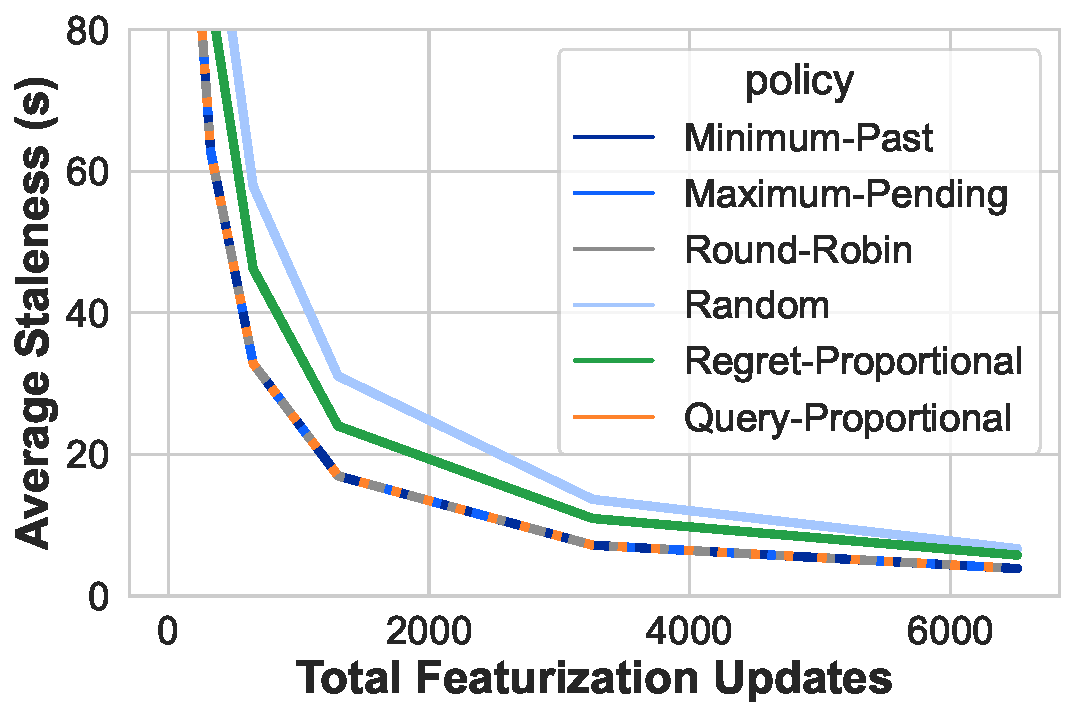
\includegraphics[width=6cm]{ralf/figures/yahoo_a1_results_line_staleness.pdf}
    \caption{\textbf{Queried feature staleness (Anomaly Detection):} Average staleness at query time across key, measured by the number of timesteps since the last update.}
    \label{fig:stl-yahoo-staleness}
\end{figure}

\subsubsection{Query Distributions} 
The Anomaly Detection workload has a uniform query distribution over keys, while for the Recommendation workload, queries for a given user typically come in bursts after long periods of inactivity. We additionally test the effect of different query distributions by re-assinging the inter-arrival times for the Recommendation workloads. We re-assign the inter-arrival times between events to follow an Exponential distribution (equivalent to a poisson process) and a Gaussian distribution, where the mean inter-arrival time is the same as the original distribution. We show in \cref{fig:als-dist} that this leads to similar results as the original distribution of data, showing that Regret-Proportional scheduling is robust to different query distributions. 

\begin{figure}[t]
     \centering
    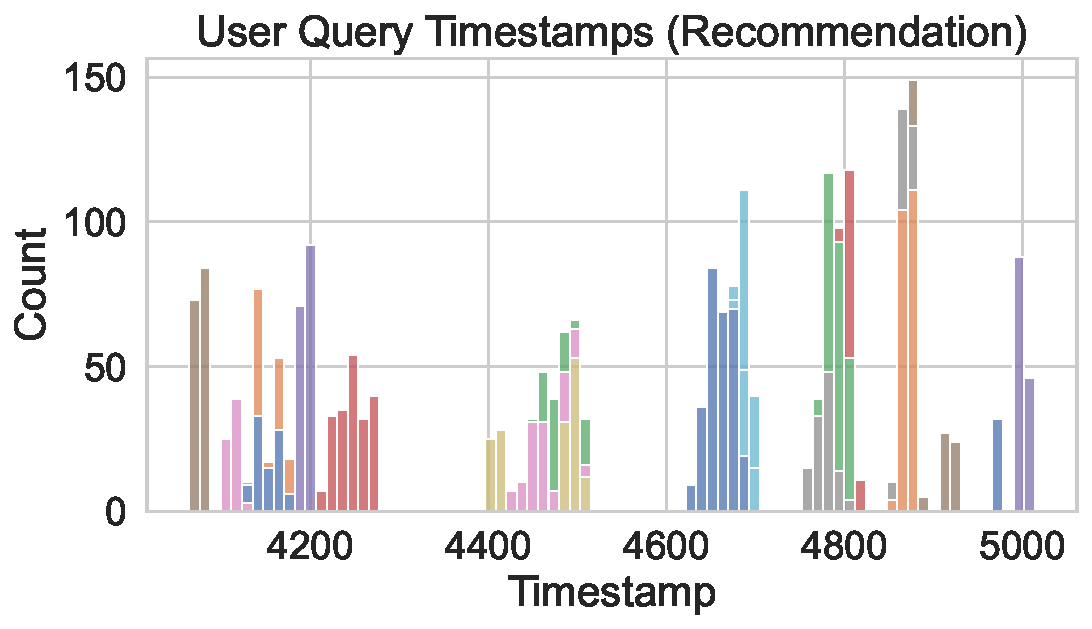
\includegraphics[width=6cm]{ralf/figures/als_user_dist.pdf}
    \caption{\textbf{Frequency of user queries over timestamps.}}
    \label{fig:als-user-dist} 
\end{figure}

\begin{figure}[t]
     \centering
    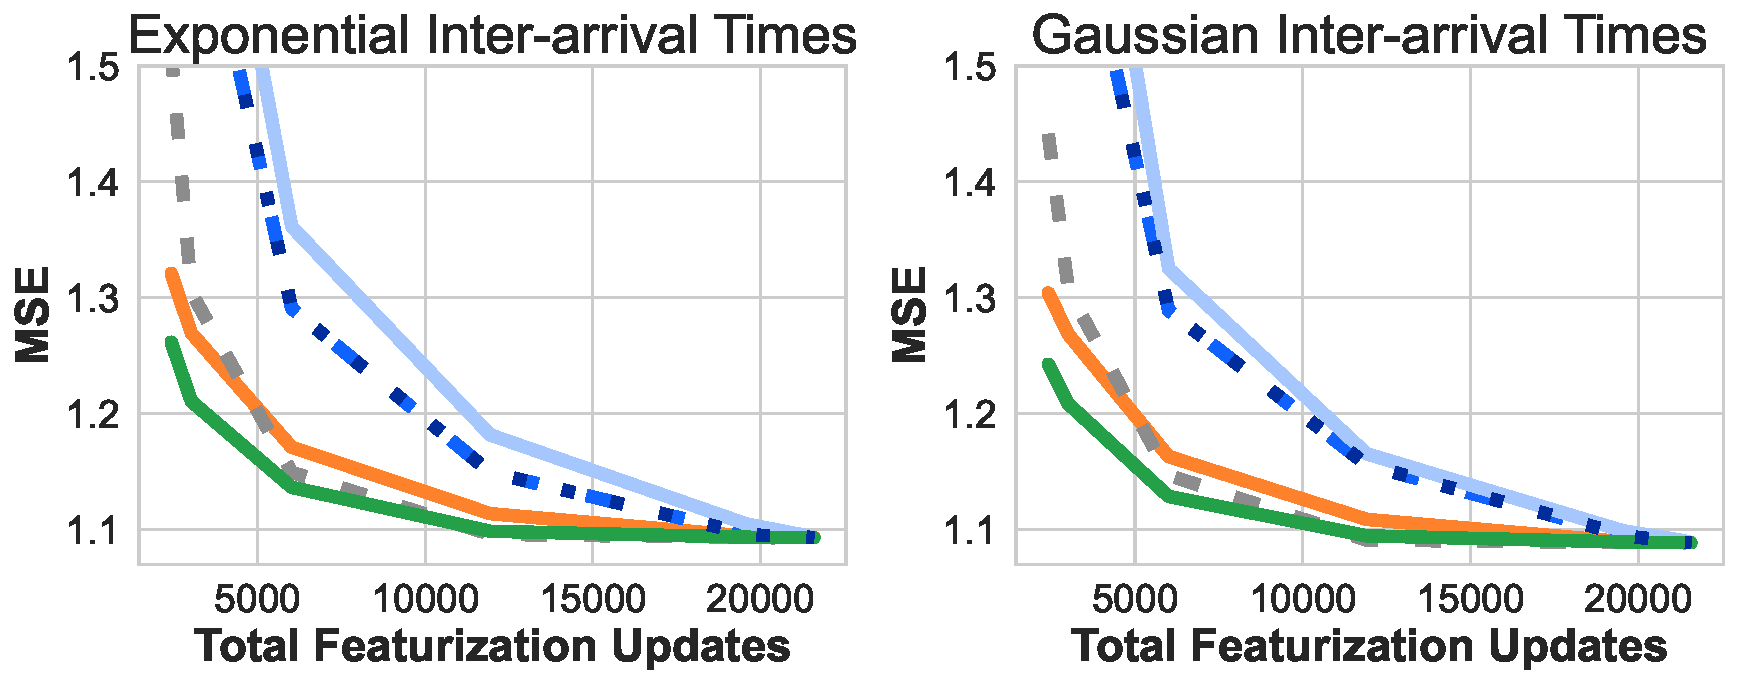
\includegraphics[width=8cm]{ralf/figures/als_dist.pdf}
    \caption{\textbf{Recommendation workload with modified query inter-arrival time shows similar results.}}
    \label{fig:als-dist} 
\end{figure}


\subsection{How well can future error be predicted?}
We evaluate how well error from past queries can predict errors in future queries as a function of the window size of the past queries considered and the lag between the error data and timestamp which we are trying to predict error for (which we refer to as the offset). We train a linear regression model on both the Recommendation and Anomaly Detection workloads to predict error for a future timestep (with some offset) given a window of previous errors for a given key. We show results in \cref{fig:predict_error}, where we plot the MSE of the predicted error. Both workloads benefit from larger windows, but is especially important for the Anomaly Detection workload. Varying the offset hurts the accuracy of the model in Recommendation, suggesting that the freshness of the feedback is critical, while Anomaly Detection relies on just having a sufficient window size (since the per-key error is much more stable over time). 
%These results suggest that the Anonomaly Detection workload could rely on offline regret estimates (described in \cref{ss:online-scheduling-error-feedback}), since the per-key regret is stable, while the Recommendation workload could not. 


\begin{figure}
    \centering
    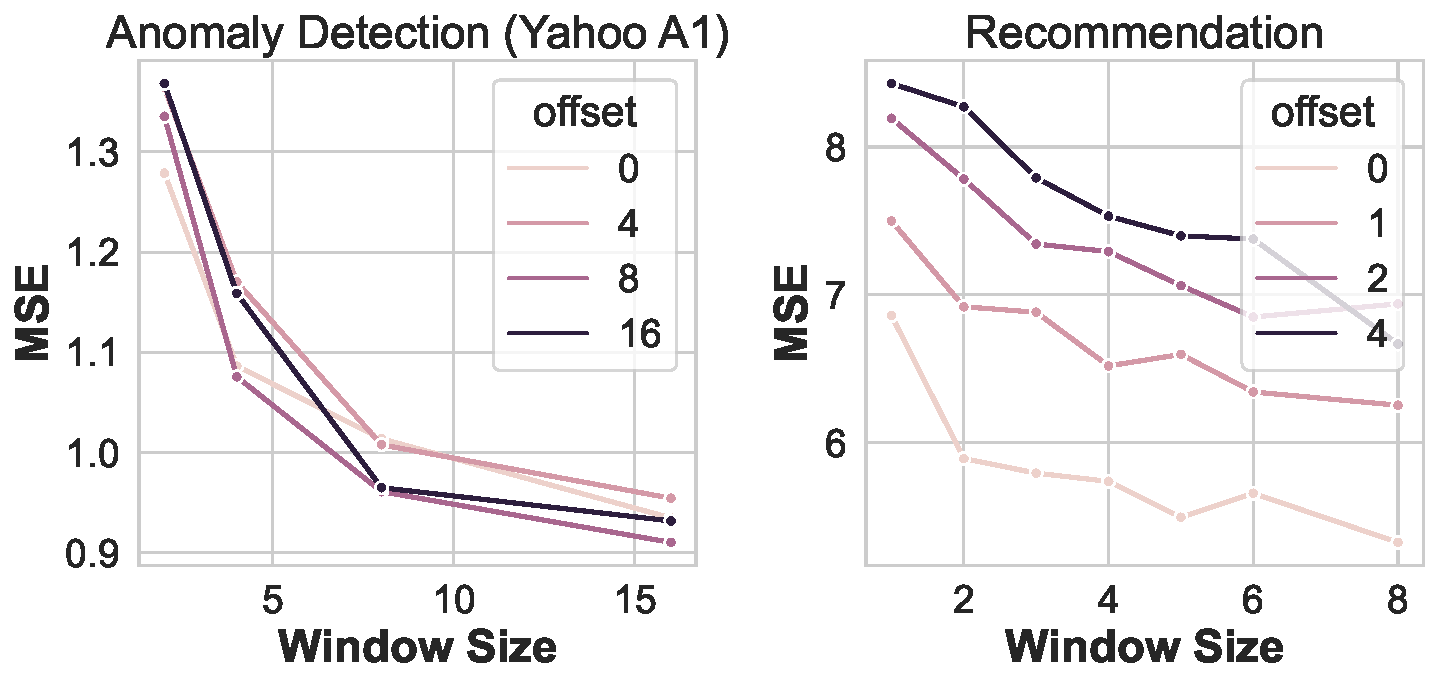
\includegraphics[width=8cm]{ralf/figures/predict_error.pdf}
    \caption{Predicting next timestep error for different window sizes (number of past errors) and offset (timestep delay of the window).}
    \label{fig:predict_error}
\end{figure}


\subsection{Regret-Proportional Scheduling Limitations}
In our workloads, we assume that that the prediction error can be observed and fed back to the scheduler; this allows us to make decisions that will minimize future prediction error by selectively updating certain features. Our purpose in this evaluation is to demonstrate that such feedback from downstream applications---providing recent prediction errors and query patterns--- can be leveraged to make better scheduling decisions for feature maintenance. We believe that future work will be able to make progress is learning to effectively estimate regret from offline data for certain workloads.

There is additionally a concern here with coverage. If we only update features that have incurred past regret, we will fail to update features that have not been queried in the past (e.g. a user who has not logged in in a long time suddenly begins a new session). Such keys form the long tail of the query distribution. To handle this concern, \system{} can be used with a higher default regret value (described in \cref{ss:default-regret}, which will ensure that sufficiently stale keys will eventually be prioritized. However, even without this, since \system{}'s policy is online, so can react quickly to prioritize features that suddenly start to get quried, as shown in our results from the Recommendation workload.


















